\documentclass[sigconf,review]{acmart}

\graphicspath{{gfx/}}

\usepackage{paralist}
\usepackage{pifont}
\usepackage{xcolor}
\usepackage{listings}
\usepackage{booktabs}
\usepackage{tabularx}
\usepackage{multirow}
\usepackage{colortbl}
\usepackage{tikz}
\usepackage{todonotes}
\usepackage{makecell}
\usepackage{float}
\usepackage{dblfloatfix}
\usepackage{placeins}
\usepackage{caption}

\usetikzlibrary{positioning, shapes.geometric, shapes.multipart, arrows.meta, fit}
\tikzset{
  classbox/.style={
    draw, rectangle split, rectangle split parts=2,
    rounded corners=2pt, font=\small, align=left,
    minimum width=3.8cm, inner sep=4pt
  },
  msLbl/.style={font=\scriptsize, midway, right, xshift=1pt},
  msLblL/.style={font=\scriptsize, midway, left, xshift=-1pt},
  enumbox/.style={
    draw, dashed, rounded corners=2pt,
    font=\scriptsize, align=left, inner sep=4pt
  },
}
\usepackage{subfig}
\usepackage{hyperref}
\usepackage{wrapfig}
\emergencystretch=1em

\definecolor{evocolor}{RGB}{198, 224, 180}
\definecolor{migcolor}{RGB}{189, 215, 238}
\newcommand{\fullmark}{\ding{51}}
\newcommand{\halfmark}{\ding{115}}

\lstdefinestyle{SMILE}{
  basicstyle=\ttfamily\small,
  keywordstyle=\bfseries,
  commentstyle=\itshape\color{gray},
  breaklines=true,
  frame=single,
  captionpos=b
}

\AtBeginDocument{%
  \providecommand\BibTeX{{%
    Bib\TeX}}}

\setcopyright{acmlicensed}
\copyrightyear{2018}
\acmYear{2018}
\acmDOI{XXXXXXX.XXXXXXX}
\acmConference[Conference acronym 'XX]{Make sure to enter the correct
  conference title from your rights confirmation email}{June 03--05,
  2018}{Woodstock, NY}
\acmISBN{978-1-4503-XXXX-X/2018/06}

\begin{document}

\title{
% SMILE: Schema Migration and Evolution Language
SMILE: A Unifying Evolution Language to Transform Schemas Across Data Models}

\author{Lu Li}
\affiliation{%
  \institution{FernUniversit\"{a}t in Hagen}
  \country{Germany}}
\email{lu.li@fernuni-hagen.de}

\author{Andr\'e Conrad}
\orcid{0000-0001-6681-2798}
\affiliation{%
  \institution{FernUniversit\"{a}t in Hagen}
  \country{Germany}}
\email{andre.conrad@fernuni-hagen.de}

\author{Dominique Hausler}
\orcid{0009-0004-2381-133X}
\affiliation{%
  \institution{University of Regensburg}
  \country{Germany}}
\email{dominique.hausler@ur.de}

\author{Uta St\"orl}
\orcid{0000-0003-2771-142X}
\affiliation{%
  \institution{FernUniversit\"{a}t in Hagen}
  \country{Germany}}
\email{uta.stoerl@fernuni-hagen.de}

\renewcommand{\shortauthors}{Li et al.}

\begin{abstract}
  Modern applications often combine relational, document, graph, and wide-column databases to serve different workloads.
  As application requirements change, schemas must often evolve within a system or be migrated across systems.
  Existing schema evolution languages are mostly limited to intra-system scenarios, while a common formal grammar spanning both intra-system evolution and inter-system migration remains underexplored.
  We present SMILE (Schema Migration and Evolution Language), a domain-specific language that addresses this gap.
  The language defines a taxonomy of schema change operations covering schema structure, constraints, and paradigm-specific constructs, formalized through an ANTLR4-based grammar.
  To operationalize SMILE, we further develop the SMILE Engine, which builds on a canonical metamodel and adopts a Hub-and-Spoke architecture to reduce inter-system mapping complexity.
  We validate the approach across all 16 migration and evolution scenarios, with 32/32 test configurations passing a two-layer validation pipeline.
  The results show that a unified language-based approach to schema evolution and migration across heterogeneous database paradigms is feasible.
\end{abstract}

\keywords{Schema Migration, Schema Evolution, Domain-Specific Language, NoSQL, Metamodel, ANTLR4}

\maketitle

% ============================================================
\section{Introduction}
\label{sec:introduction}
% ============================================================

Heterogeneous data architectures have become common in modern applications, where different workloads are often served by different data models. For example, Sega reported a migration from an RDBMS to MongoDB to improve performance~\cite{bansal2021journey}. In such environments, schema change is required both within individual systems and across system boundaries. SMILE targets four database paradigms: relational, document, graph, and wide-column. These paradigms differ substantially in how they represent structure and relationships, which makes unified schema change support challenging.


\emph{Schema evolution} refers to modifying a schema within the same database system (intra-system)~\cite{brahmia2024literature}, while
\emph{schema migration} refers to transforming a schema between different database systems (inter-system)~\cite{googlecloud2024heterogeneous}.
For the four paradigms considered in this work, this results in 4 evolution scenarios on the diagonal and 12 migration scenarios off the diagonal, i.e., 16 scenarios in total (Table~\ref{tab:migration-matrix}).


Existing schema evolution languages are mostly limited to intra-system scenarios~\cite{storl2022darwin, chillon2022taxonomy, curino2008graceful,
herrmann2015codel, herrmann2017living, hausler2023language}, while inter-system migration work~\cite{meier2023datenmigration} addresses cross-paradigm structural transformations. Because these lines of work rely on different operation sets and are not expressed in a shared grammar, they do not directly yield a unified DSL for both evolution and migration.

To address this gap, we present \textbf{SMILE}, a domain-specific language that supports both schema evolution (intra-system) and schema migration (inter-system) within a single ANTLR4-based grammar. Rather than combining existing approaches unchanged, SMILE organizes evolution operations from the Orion taxonomy~\cite{chillon2022taxonomy}, structural transformation operations from prior work within our research group, and additional key and constraint operations into a unified taxonomy of schema change primitives.

To operationalize SMILE, we develop a prototype implementation referred to as the \textbf{SMILE Engine}. The engine uses M-Model\textsuperscript{+} as a canonical representation and adopts a Hub-and-Spoke architecture with adapters for PostgreSQL, MongoDB, Neo4j, and Cassandra. This design replaces point-to-point schema mappings with transformations through a shared metamodel, reducing the number of required mappings from $O(N^2)$ to $O(N)$. It thereby makes a single language-based approach feasible across all 16 migration and evolution scenarios.

% \begin{figure}[htbp]
%   \centering
%   \includegraphics[width=\columnwidth]{{overview.drawio}.pdf}
%   \caption{Overview of the SMILE language and engine.}
%   \label{fig:SMILE-overview}
% \end{figure}

\paragraph{Contributions.}
SMILE focuses on schema-level change and does not address data migration or runtime query rewriting.
Within this scope, we make four contributions:
\begin{compactitem}
    \item A \textbf{unified taxonomy of schema change primitives} that brings together schema evolution and schema migration operations within a single operation model, together with two ANTLR4-based grammar variants for expressing these changes across all 16 migration and evolution scenarios.

    \item An \textbf{extended canonical metamodel, M-Model\textsuperscript{+}}, which refines the M-Model~\cite{conrad2022metamodels} with the constructs required for cross-paradigm schema migration and serves as the hub representation of the approach.

    \item A \textbf{prototype framework, the SMILE Engine}, which realizes the language through a Hub-and-Spoke architecture while providing execution, validation, and interactive web-based visualization for PostgreSQL, MongoDB, Neo4j, and Cassandra.

    \item A \textbf{comprehensive validation and evaluation} across the full $4 \times 4$ scenario matrix, covering 32 test configurations based on two grammar variants for each of the 16 directions, with all configurations passing both validation layers.
\end{compactitem}

% ============================================================
\section{Related Work}
\label{sec:related-work}
% ============================================================

The following paragraphs review prior work on schema matching and mapping, schema evolution, schema migration, and evolution languages.
\todo[inline]{add work on constraints e.g. PG-Keys \cite{DBLP:conf/sigmod/AnglesBDFHHLLLM21,DBLP:conf/kcap/TomaszukG25}}


\paragraph{Schema Matching \& Mapping.}
Schema migration presupposes schema matching and mapping, since source and target structures must be related before transformations can be specified. A widely used categorization of schema matching techniques is given in~\cite{DBLP:journals/vldb/RahmB01}. Mapping strategies across data models are discussed in~\cite{DBLP:conf/idt2/CeresnakDMK21,DBLP:journals/sp/AftabIABA20,DBLP:journals/kais/BansalSA24}, while graph-based and pattern-based approaches are presented in~\cite{DBLP:journals/dpd/DingSW20,DBLP:journals/pvldb/MartensNPRVV23, DBLP:conf/icdt/Barcelo0R13,DBLP:conf/pods/FrancisL17}. These works address how correspondences between schemas are identified, whereas the present work focuses on a unified language for expressing the resulting schema changes.


\paragraph{Schema Evolution.}
Schema evolution addresses the adaptation of database schemas to changing application requirements. In relational settings, this line of work is closely related to schema modification operations such as \texttt{ALTER TABLE}. Recent model-driven work such as EvolveDB~\cite{eckwert2025evolvedb} reverse-engineers schemas into a UML-like representation and derives migration scripts from it. Related work on semantic lifting studies how low-level model differences can be transformed into higher-level change descriptions, such as semantic change sets, in the context of model versioning~\cite{DBLP:conf/kbse/KehrerKT11,DBLP:conf/icsm/KehrerKOS12}. Although these approaches are not database-specific, they are relevant here because they demonstrate how atomic differences can be abstracted into semantic change operations.

With the rise of NoSQL systems, schema evolution research expanded beyond the relational paradigm. Scherzinger, Klettke, and St\"orl~\cite{scherzinger2013managing} introduced a declarative evolution language and distinguished between eager and lazy migration strategies, while Holubov\'a, Klettke, and St\"orl~\cite{holubova2019evolution} discuss corresponding challenges in multi-model settings. For specific paradigms, MoDEvo~\cite{suarez2025data} targets column-family evolution through model transformations, Hausler et al.~\cite{hausler2023language} define evolution operations for graph databases, and Chabin et al.~\cite{DBLP:journals/ijwis/ChabinEFH21} study RDF evolution through graph rewriting rules.

In addition, prior work within our research group introduces structural transformation operations such as \texttt{NEST}, \texttt{FLATTEN}, \texttt{LINKING}, and \texttt{UNWIND} for schema restructuring across heterogeneous systems~\cite{meier2023datenmigration}. This work reuses basic evolution operations from earlier evolution proposals~\cite{scherzinger2013managing, holubova2019evolution}, but extends them with transformation-specific operations required for cross-paradigm migration.

\textit{Across the reviewed work, schema evolution and schema migration remain modeled through separate operation sets and formalisms. What is still lacking is a common taxonomy and grammar that cover both intra-system evolution and inter-system structural transformations.}

\paragraph{Evolution Languages.}
Model Management~2.0~\cite{bernstein2007model} introduced generic operators for manipulating schemas and mappings and thus established an important foundation for formal schema transformation. Building on this idea, PRISM~\cite{curino2008graceful} proposed Schema Modification Operators (SMOs) for relational schema evolution and additionally supported automatic query rewriting. PRIMA~\cite{moon2009prima} extended this line of work toward temporal querying over evolving schemas, while CoDEL~\cite{herrmann2015codel} and BiDEL~\cite{herrmann2017living} further developed the relational setting toward relational completeness and bidirectional propagation across co-existing schema versions.

With the rise of NoSQL and multi-model systems, evolution language research moved beyond the relational paradigm. Holubov\'a, Klettke, and St\"orl~\cite{holubova2019evolution} identified key challenges for multi-model evolution and outlined an EBNF syntax for a corresponding language. Orion~\cite{chillon2022taxonomy}, grounded in U-Schema~\cite{candel2022unified}, organizes schema change operations for NoSQL databases into five categories and implements them as a platform-independent DSL. Darwin~\cite{storl2022darwin} complements this perspective with a data platform for schema evolution management, including schema version tracking and migration support. For graph databases specifically, Hausler et al.~\cite{hausler2023language} define evolution operations in an EBNF-like grammar with an implementation in Neo4j.

\textit{These languages formalize schema evolution precisely, but their grammars remain tied to particular paradigms or intra-system settings. Their abstractions therefore do not transfer directly to cross-paradigm migration scripts.}

\paragraph{Schema Transformation.}
Schema transformation generalizes schema evolution to changes between different source and target schemas and therefore depends on schema matching and mapping to relate their structures. Existing work in this area often focuses on specific model pairs or transformation settings. For example, Rabbani et al.~\cite{DBLP:journals/pacmmod/RabbaniLBH24} present a transformation strategy between RDF and property graphs, while Hausler et al.~\cite{DBLP:conf/er/HauslerEKGT25} propose a model-driven, GQL-conform transformation approach between versions of property graph schemas. Other work adopts a metamodel-based perspective for schema transformation, for instance in UMLtoNoSQL~\cite{DBLP:conf/aiccsa/AbdelhediBAZ17}. In the context of property graphs, Bonifati~\cite{DBLP:journals/pvldb/Bonifati25}, building on PG-Schema~\cite{DBLP:journals/pacmmod/AnglesBD0GHLLMM23}, discusses a declarative approach for expressing transformations and integrating data into property graphs.

\textit{These studies show that schema transformation can be specified effectively for particular model pairs, standards, or metamodel-driven settings. What they do not yet offer is a language layer that spans both intra-system evolution and cross-paradigm migration across heterogeneous database paradigms.}


\paragraph{Constraints.}
Recent work has formalized key and constraint concepts in the property-graph setting. PG-Keys~\cite{DBLP:conf/sigmod/AnglesBDFHHLLLM21} proposes a flexible framework for key constraints in property graphs, introducing the modes \emph{exclusive}, \emph{mandatory}, and \emph{singleton} for nodes, edges, and properties as part of the GQL standardization effort. Tomaszuk and Labra Gayo~\cite{DBLP:conf/kcap/TomaszukG25} further extend PG-Schema with property constraints.

\textit{This line of work formalizes keys and constraints rigorously at the schema level. In the current literature, however, these notions remain largely bound to the graph paradigm rather than being generalized into a common cross-paradigm operation layer.}

\paragraph{Metamodels.}
A canonical hub for cross-paradigm schema transformation requires a central, platform-independent metamodel. Several metamodels have been proposed for multi-model database systems~\cite{atzeni2020data, abdelhedi2017umltonosql, vanhove2017data, mali2020modeldrivenguide, zdepski2020pddm, candel2022unified, conrad2022metamodels}. Among them, U-Schema~\cite{candel2022unified} and the M-Model~\cite{conrad2022metamodels} are the most relevant to this work because both cover the four database paradigms targeted by SMILE and provide sufficiently rich structural abstractions for cross-paradigm representation (Table~\ref{tab:metamodel-comparison-rw}).

U-Schema is a unified logical metamodel for relational, document, graph, key-value, and columnar systems. It introduces \texttt{StructuralVariation}s to capture schema-on-read variability and distinguishes between structural and logical features. However, concepts such as \texttt{Aggregate} and \texttt{Reference} are represented in separate branches of its feature hierarchy.

\textit{Compared with U-Schema, the M-Model offers a more suitable starting point for SMILE because its relationship hierarchy and explicit key typing align more directly with cross-paradigm transformation requirements. At the same time, the present work requires additional constructs beyond the original model, which motivates the extension to M-Model\textsuperscript{+}.}

\begin{table}[h!]
  \centering
  \caption{Comparison of U-Schema and M-Model as candidate canonical metamodels}
  \label{tab:metamodel-comparison-rw}
  \renewcommand{\arraystretch}{1.25}
  \setlength{\tabcolsep}{3pt}
  \scriptsize
  \begin{tabular}{@{}
    >{\bfseries\raggedright\arraybackslash}p{1.8cm}
    >{\raggedright\arraybackslash}p{3.2cm}
    >{\raggedright\arraybackslash}p{3.2cm}
  @{}}
  \toprule
  \rowcolor{gray!15}
  \textbf{Criterion} &
  \textbf{U-Schema}~\cite{candel2022unified} &
  \textbf{M-Model}~\cite{conrad2022metamodels} \\
  \midrule
  Purpose &
  Universal metamodel for DB engineering (migration, visualization, query optimization) &
  Metamodel for schema and data migration between heterogeneous DB systems \\
  \addlinespace
  Relationship Hierarchy &
  No common superclass (Reference $\to$ LogicalFeature; Aggregate $\to$ StructuralFeature) &
  Unified superclass: Relationship $\to$ Reference, Embedded, Edge \\
  \addlinespace
  Key Modeling &
  Generic set of attributes, no type distinction &
  Explicit \texttt{keyType} (partition, clustering) for composite keys \\
  \addlinespace
  Structural Variations &
  First-class concept with Full Variability and Union Schema modes &
  Not supported; single fixed structure per EntityType \\
  \addlinespace
  Graph Support &
  \texttt{RelationshipType} as first-class schema type with own variations &
  \texttt{Edge} subclass of Relationship + separate \texttt{RelationshipType} class \\
  \addlinespace
  Design Philosophy &
  Comprehensive, high complexity &
  Minimal complexity, migration-focused \\
  \bottomrule
  \end{tabular}
\end{table}

\paragraph{Summary of Research Gaps.}
Across the reviewed literature, schema evolution and schema
migration are still described through separate operation sets
and grammars, with no shared language framework connecting them.
Keys, constraints, and paradigm-specific schema constructs
likewise lack a common operation layer across the four database
paradigms considered here. At the tool level, existing systems
support individual parts of the process but do not yet combine
a canonical hub representation, systematic validation, and
interactive support for cross-paradigm schema change in one
environment. These gaps motivate the design of SMILE as a
common foundation for language design, metamodel-based
representation, and tool support.


\section{SMILE Language}
\label{sec:operation-taxonomy}

SMILE organizes schema change operations into a taxonomy of atomic primitives.
The taxonomy brings together evolution operations from the reviewed approaches and structural transformation operations from prior work within our research group into seven categories.
Table~\ref{tab:terminology-comparison} aligns the terminology used across prior approaches, and Table~\ref{tab:operation-comparison} compares their operation coverage with SMILE.

Four design principles guide the syntax.
Structural operations are organized as \textbf{symmetric inverse pairs}, where each forward operation has a corresponding reverse (NEST\,/\,UNNEST, FLATTEN\,/\,UNFLATTEN, WIND\,/\,UNWIND), enabling bidirectional scripts.
Operations also follow a \textbf{consistent naming scheme}: creation operations begin with \texttt{ADD\_*}, removal operations with \texttt{DELETE\_*}, and type conversions with \texttt{CAST\_*}.
SMILE further provides \textbf{two grammar variants}. The Specific grammar uses one keyword per operation (e.g., \texttt{ADD\_ENTITY}), whereas the Generalized grammar combines verb and object tokens (e.g., \texttt{ADD ENTITY}). Both variants are translated into the same internal operation representation.
Finally, SMILE uses \textbf{explicit operation sequences}, so that each transformation step remains directly visible in the script.

For instance, a single \texttt{UNNEST} statement can extract a deeply nested embedded structure from \texttt{orders} into a separate entity \texttt{order\_details}, including nested product, category, supplier, and address levels, while establishing a foreign-key link through a \texttt{WITH \ldots\ TO} clause.

\begin{table}[h!]\todo{color code SMILE in lightblue!!!}
\centering
\caption{Terminology mapping of core schema concepts across existing approaches and SMILE}
\label{tab:terminology-comparison}
\renewcommand{\arraystretch}{1.15}
\setlength{\tabcolsep}{2pt}
\scriptsize
\begin{tabular}{ccccc
  >{\columncolor{blue!10}}p{0.9cm}c}
\toprule
\rowcolor{gray!15}
\textbf{Concept} &
\textbf{PRISM \cite{curino2008graceful}} &
\textbf{Darwin \cite{storl2022darwin}} &
\textbf{Orion \cite{chillon2022taxonomy}} &
\textbf{GEO \cite{hausler2023language}} &
\textbf{SMILE} \\
\rowcolor{gray!15}
& \textbf{CoDEL \cite{herrmann2015codel}} & & & &\\
\rowcolor{gray!15}
& \textbf{BiDEL \cite{herrmann2017living}} & & & &\\
\midrule
Entity Type & Table / Relation & Type & Schema Type & Entity Type & Entity Type \\
Property & Column / Attribute & Property & Feature & Property & Property \\
Embed. & --- &--- &Aggregate &--- &Embedded \\
Ref. &Foreign Key &--- &Reference &Relationship &Reference \\
\bottomrule
\end{tabular}
\end{table}

\todo[inline]{all evolution languages??, what is prior work?}
% ============================================================
% Full-width Operation Comparison Table
% ============================================================
% \begin{table*}[htbp]
% \centering
% \caption{Comparison of schema evolution and migration operations across existing approaches and SMILE}
% \label{tab:operation-comparison}
% \renewcommand{\arraystretch}{1.05}
% \setlength{\tabcolsep}{2pt}
% \tiny
% \begin{tabular}{
%   |>{\raggedright\arraybackslash}p{1.2cm}
%   |>{\raggedright\arraybackslash}p{1.6cm}
%   |>{\raggedright\arraybackslash}p{2.4cm}
%   |c|c|c|c|c|c|c
%   |>{\raggedright\arraybackslash}p{2.2cm}
%   |>{\raggedright\arraybackslash}p{2.2cm}|
% }
% \hline
%   \multicolumn{1}{|c|}{\raisebox{1.2em}{\textbf{Category}}} &
%   \multicolumn{1}{c|}{\raisebox{1.2em}{\textbf{Operation}}} &
%   \multicolumn{1}{c|}{\raisebox{1.2em}{\textbf{Description}}} &
%   \rotatebox{70}{\textbf{PRISM}} &
%   \rotatebox{70}{\textbf{CoDEL}} &
%   \rotatebox{70}{\textbf{BiDEL}} &
%   \rotatebox{70}{\textbf{Darwin}} &
%   \rotatebox{70}{\textbf{Orion}} &
%   \rotatebox{70}{\textbf{GEO}} &
%   \rotatebox{70}{\textbf{Prior Work}} &
%   \multicolumn{1}{c|}{\raisebox{1.2em}{\textbf{SMILE Specific}}} &
%   \multicolumn{1}{c|}{\raisebox{1.2em}{\textbf{SMILE General.}}} \\

% \hline
% \multirow{8}{1.2cm}{Entity\newline Type\newline Ops}
%   & Add Entity Type        & Create a new entity type           & \checkmark & \checkmark & \checkmark & \checkmark & \checkmark & \checkmark & --- & \texttt{ADD\_ENTITY}     & \texttt{ADD ENTITY} \\
% \cline{2-12}
%   & Delete Entity Type     & Remove an entity type and its data & \checkmark & \checkmark & \checkmark & \checkmark & \checkmark & \checkmark & --- & \texttt{DELETE\_ENTITY}  & \texttt{DELETE ENTITY} \\
% \cline{2-12}
%   & Rename Entity Type     & Change entity type name            & \checkmark & \checkmark & \checkmark & \checkmark & \checkmark & \checkmark & --- & \texttt{RENAME\_ENTITY}  & \texttt{RENAME ENTITY} \\
% \cline{2-12}
%   & Copy Entity Type       & Duplicate entity type structure    & \checkmark & \checkmark$^{a}$ & \checkmark$^{a}$ & --- & --- & \checkmark & --- & \texttt{COPY\_ENTITY}    & \texttt{COPY ENTITY} \\
% \cline{2-12}
%   & Merge Entity Types    & Combine two entity types into one & \checkmark & \checkmark & \checkmark & \checkmark & \checkmark & \checkmark & \checkmark & \texttt{MERGE}     & \texttt{MERGE} \\
% \cline{2-12}
%   & Split Entity Type      & Partition by attr.\ subsets   & \checkmark & \checkmark & via dec. & \checkmark & \checkmark & \checkmark & \checkmark & \texttt{SPLIT}     & \texttt{SPLIT} \\
% \cline{2-12}
%   & Extract Entity Type    & Derive from selected features & --- & --- & --- & --- & \checkmark & --- & --- & via \texttt{SPLIT}       & via \texttt{SPLIT} \\
% \cline{2-12}
%   & Cast Entity Type       & Change entity type kind       & --- & --- & --- & --- & --- & --- & --- & \texttt{CAST\_ENTITY}    & \texttt{CAST ENTITY} \\
% \hline
% \multirow{8}{1.2cm}{Property\newline Ops}
%   & Add Property      & Add a new attribute           & \checkmark & \checkmark & \checkmark & \checkmark & \checkmark & \checkmark & \checkmark & \texttt{ADD\_ATTRIBUTE}     & \texttt{ADD ATTRIBUTE} \\
% \cline{2-12}
%   & Delete Property   & Remove an attribute           & \checkmark & \checkmark & \checkmark & \checkmark & \checkmark & \checkmark & \checkmark & \texttt{DELETE\_ATTRIBUTE}  & \texttt{DELETE ATTRIBUTE} \\
% \cline{2-12}
%   & Rename Property   & Change attribute name         & \checkmark & \checkmark & \checkmark & \checkmark & \checkmark & \checkmark & \checkmark & \texttt{RENAME\_ATTRIBUTE}  & \texttt{RENAME ATTRIBUTE} \\
% \cline{2-12}
%   & Copy Property     & Duplicate an attribute        & --- & --- & --- & \checkmark & \checkmark & \checkmark & \checkmark & \texttt{COPY\_ATTRIBUTE}    & \texttt{COPY ATTRIBUTE} \\
% \cline{2-12}
%   & Move Property     & Move attr.\ to other entity   & --- & --- & --- & \checkmark & \checkmark & \checkmark & \checkmark & \texttt{MOVE\_ATTRIBUTE}    & \texttt{MOVE ATTRIBUTE} \\
% \cline{2-12}
%   & Cast / Type Change & Change data type             & ---$^{b}$ & --- & --- & --- & \checkmark & --- & --- & \texttt{CAST\_ATTRIBUTE}    & \texttt{CAST ATTRIBUTE} \\
% \cline{2-12}
%   & Promote           & Mark as key attribute         & --- & --- & --- & --- & \checkmark & --- & --- & via \texttt{ADD\_PRIMARY\_KEY} & via \texttt{ADD PRIM.\ KEY} \\
% \cline{2-12}
%   & Demote            & Unmark as key attribute       & --- & --- & --- & --- & \checkmark & --- & --- & via \texttt{DEL\_PRIMARY\_KEY} & via \texttt{DEL PRIM.\ KEY} \\
% \hline
% \multirow{7}{1.2cm}{Structural\newline Transform.}
%   & Flatten           & Nested $\rightarrow$ parent fields        & --- & --- & --- & --- & via unnest & --- & \checkmark & \texttt{FLATTEN}     & \texttt{FLATTEN} \\
% \cline{2-12}
%   & Unflatten         & Flat $\rightarrow$ nested object          & --- & --- & --- & --- & via nest   & --- & ---        & \texttt{UNFLATTEN}   & \texttt{UNFLATTEN} \\
% \cline{2-12}
%   & Unnest            & Embedded $\rightarrow$ separate entity    & --- & --- & --- & --- & morph aggr$\rightarrow$ref & --- & --- & \texttt{UNNEST} & \texttt{UNNEST} \\
% \cline{2-12}
%   & Nest              & Entity $\rightarrow$ embedded struct.     & --- & --- & --- & --- & morph ref$\rightarrow$aggr & --- & \checkmark & \texttt{NEST}  & \texttt{NEST} \\
% \cline{2-12}
%   & Unwind            & Array $\rightarrow$ individual entities   & --- & --- & --- & --- & ---        & --- & \checkmark & \texttt{UNWIND}      & \texttt{UNWIND} \\
% \cline{2-12}
%   & Wind              & Rows $\rightarrow$ array                  & --- & --- & --- & --- & ---        & --- & ---        & \texttt{WIND}        & \texttt{WIND} \\
% \cline{2-12}
%   & Linking           & Create ref.\ by join cond.               & --- & --- & --- & --- & ---        & --- & \checkmark & via \texttt{WIND}    & via \texttt{WIND} \\
% \hline
% \multirow{5}{1.2cm}{Reference\newline Ops}
%   & Add Reference       & Add a reference             & --- & --- & --- & --- & \checkmark & --- & --- & \texttt{ADD\_CONSTRAINT}    & \texttt{ADD CONSTR.} \\
% \cline{2-12}
%   & Delete Reference    & Remove a reference          & --- & --- & --- & --- & \checkmark & --- & --- & \texttt{DELETE\_CONSTRAINT} & \texttt{DELETE CONSTR.} \\
% \cline{2-12}
%   & Cast Reference      & Change constraint type      & --- & --- & --- & --- & \checkmark & --- & --- & \texttt{CAST\_CONSTRAINT}   & \texttt{CAST CONSTR.} \\
% \cline{2-12}
%   & Multiplicity Change & Change cardinality          & --- & --- & --- & --- & \checkmark & --- & --- & \texttt{RECARD}             & \texttt{RECARD} \\
% \cline{2-12}
%   & Morph (Ref$\rightarrow$Aggr) & Ref.\ $\rightarrow$ embedded aggr. & --- & --- & --- & --- & \checkmark & --- & --- & via \texttt{NEST} & via \texttt{NEST} \\
% \hline
% \multirow{3}{1.2cm}{Aggr./\newline Emb.\ Ops}
%   & Add Embedded       & Add embedded struct.          & --- & --- & --- & --- & \checkmark & --- & --- & \texttt{ADD\_EMBEDDED}    & \texttt{ADD EMBEDDED} \\
% \cline{2-12}
%   & Delete Embedded    & Remove embedded struct.       & --- & --- & --- & --- & \checkmark & --- & --- & \texttt{DELETE\_EMBEDDED} & \texttt{DELETE EMBEDDED} \\
% \cline{2-12}
%   & Morph (Aggr$\rightarrow$Ref) & Embedded $\rightarrow$ reference & --- & --- & --- & --- & \checkmark & --- & --- & via \texttt{UNNEST} & via \texttt{UNNEST} \\
% \hline
% \multirow{7}{1.2cm}{Key/\newline Constr.\newline Ops}
%   & Add Primary Key     & Define primary key          & --- & --- & --- & --- & --- & --- & --- & \texttt{ADD\_PRIMARY\_KEY}      & \texttt{ADD PRIM.\ KEY} \\
% \cline{2-12}
%   & Add Foreign Key     & Define foreign key          & --- & --- & --- & --- & --- & --- & --- & \texttt{ADD\_FOREIGN\_KEY}      & \texttt{ADD FOR.\ KEY} \\
% \cline{2-12}
%   & Add Unique Key      & Define unique constraint    & --- & --- & --- & --- & --- & --- & --- & \texttt{ADD\_UNIQUE\_KEY}       & \texttt{ADD UNIQ.\ KEY} \\
% \cline{2-12}
%   & Add Partition Key   & Define partition key        & --- & --- & --- & --- & --- & --- & --- & \texttt{ADD\_PARTITION\_KEY}    & \texttt{ADD PART.\ KEY} \\
% \cline{2-12}
%   & Add Clustering Key  & Define clustering key       & --- & --- & --- & --- & --- & --- & --- & \texttt{ADD\_CLUSTERING\_KEY}   & \texttt{ADD CLUST.\ KEY} \\
% \cline{2-12}
%   & Delete Prim./For./Uniq. & Remove key constraint   & --- & --- & --- & --- & --- & --- & --- & \texttt{DELETE\_*\_KEY}         & \texttt{DELETE *~KEY} \\
% \cline{2-12}
%   & Delete Part./Clust. & Remove partition/clust.\ key & --- & --- & --- & --- & --- & --- & --- & \texttt{DELETE\_*\_KEY}         & \texttt{DELETE *~KEY} \\
% \hline
% \multirow{6}{1.2cm}{Graph-\newline specific\newline Ops}
%   & Add RelType         & Add relationship type       & --- & --- & --- & --- & \checkmark & \checkmark & --- & via \texttt{ADD\_ENTITY}   & via \texttt{ADD ENTITY} \\
% \cline{2-12}
%   & Delete RelType      & Delete relationship type    & --- & --- & --- & --- & \checkmark & \checkmark & --- & via \texttt{DEL.\_ENTITY}  & via \texttt{DEL.\ ENTITY} \\
% \cline{2-12}
%   & Rename RelType      & Rename relationship type    & --- & --- & --- & --- & \checkmark & \checkmark & --- & via \texttt{REN.\_ENTITY}  & via \texttt{REN.\ ENTITY} \\
% \cline{2-12}
%   & Add Label           & Add a node label            & --- & --- & --- & --- & --- & \checkmark & --- & \texttt{ADD\_LABEL}            & \texttt{ADD LABEL} \\
% \cline{2-12}
%   & Delete Label        & Remove a node label         & --- & --- & --- & --- & --- & \checkmark & --- & \texttt{DELETE\_LABEL}         & \texttt{DELETE LABEL} \\
% \cline{2-12}
%   & Transform           & Node $\leftrightarrow$ Relationship     & --- & --- & --- & --- & --- & \checkmark & --- & \texttt{TRANSFORM}      & \texttt{TRANSFORM} \\
% \hline
% \multicolumn{3}{|l|}{\cellcolor{gray!10}\textbf{Scope}} &
% \multicolumn{3}{c|}{\cellcolor{gray!10}Intra (Rel.)} &
% \multicolumn{2}{c|}{\cellcolor{gray!10}Intra (NoSQL)} &
% \cellcolor{gray!10}Intra (Graph) &
% \cellcolor{gray!10}Inter &
% \multicolumn{2}{c|}{\cellcolor{gray!10}\textbf{Both}} \\
% \hline
% \multicolumn{12}{|l|}{\parbox{0.95\linewidth}{\vspace{2pt}\scriptsize
% $^{a}$ CoDEL: via \texttt{Split\textsubscript{row}}; BiDEL: via \texttt{DECOMPOSE}.\quad
% $^{b}$ PRISM: via \texttt{ADD COLUMN \ldots\ AS func()}.\\
% Variation operations (Orion) are out of scope for SMILE.
% CoDEL additionally defines row/column-level operations outside this comparison.\vspace{2pt}}} \\
% \hline
% \end{tabular}
% \end{table*}

\begin{table*}[h!]
\centering
\caption{Comparison of schema evolution and migration operations across existing approaches and SMILE}
\label{tab:operation-comparison}
% \renewcommand{\arraystretch}{1.05}
% \setlength{\tabcolsep}{2pt}
% \tiny
\resizebox{\textwidth}{!}{
\begin{tabular}{|l|l|l|c|c|c|c|c|c|>{\columncolor{blue!10}}l|}
\hline
  \multicolumn{1}{|c|}{\textbf{Category}}&
  \multicolumn{1}{c|}{\textbf{Operation}}&
  \multicolumn{1}{c|}{\textbf{Description}}&
  \rotatebox{70}{\textbf{PRISM}} &
  \rotatebox{70}{\textbf{CoDEL}} &
  \rotatebox{70}{\textbf{BiDEL}} &
  \rotatebox{70}{\textbf{Darwin}} &
  \rotatebox{70}{\textbf{Orion}} &
  \rotatebox{70}{\textbf{GEO}} &
  \multicolumn{1}{c|}{\textbf{SMILE}}\\

\hline
\multirow{8}{*}{Entity Type Ops}
  & Add Entity Type        & Create a new entity type           & \checkmark & \checkmark & \checkmark & \checkmark & \checkmark & \checkmark & \texttt{ADD\_ENTITY}\\
\cline{2-10}
  & Delete Entity Type     & Remove an entity type and its data & \checkmark & \checkmark & \checkmark & \checkmark & \checkmark & \checkmark & \texttt{DELETE\_ENTITY} \\
\cline{2-10}
  & Rename Entity Type     & Change entity type name            & \checkmark & \checkmark & \checkmark & \checkmark & \checkmark & \checkmark & \texttt{RENAME\_ENTITY}  \\
\cline{2-10}
  & Copy Entity Type       & Duplicate entity type structure    & \checkmark & \checkmark$^{a}$ & \checkmark$^{a}$ & --- & --- & \checkmark & \texttt{COPY\_ENTITY}\\
\cline{2-10}
  & Merge Entity Types    & Combine two entity types into one & \checkmark & \checkmark & \checkmark & \checkmark & \checkmark & \checkmark & \texttt{MERGE}  \\
\cline{2-10}
  & Split Entity Type      & Partition by attr.\ subsets   & \checkmark & \checkmark & via dec. & \checkmark & \checkmark & \checkmark & \texttt{SPLIT} \\
\cline{2-10}
  & Extract Entity Type    & Derive from selected features & --- & --- & --- & --- & \checkmark & --- &  via \texttt{SPLIT} \\
\cline{2-10}
  & Cast Entity Type       & Change entity type kind       & --- & --- & --- & --- & --- & --- & \texttt{CAST\_ENTITY} \\
\hline
\multirow{8}{*}{Property\newline Ops}
  & Add Property      & Add a new attribute           & \checkmark & \checkmark & \checkmark & \checkmark & \checkmark & \checkmark & \texttt{ADD\_ATTRIBUTE}\\
\cline{2-10}
  & Delete Property   & Remove an attribute           & \checkmark & \checkmark & \checkmark & \checkmark & \checkmark & \checkmark &  \texttt{DELETE\_ATTRIBUTE} \\
\cline{2-10}
  & Rename Property   & Change attribute name         & \checkmark & \checkmark & \checkmark & \checkmark & \checkmark & \checkmark &  \texttt{RENAME\_ATTRIBUTE} \\
\cline{2-10}
  & Copy Property     & Duplicate an attribute        & --- & --- & --- & \checkmark & \checkmark & \checkmark &  \texttt{COPY\_ATTRIBUTE}  \\
\cline{2-10}
  & Move Property     & Move attr.\ to other entity   & --- & --- & --- & \checkmark & \checkmark & \checkmark &  \texttt{MOVE\_ATTRIBUTE} \\
\cline{2-10}
  & Cast / Type Change & Change data type             & ---$^{b}$ & --- & --- & --- & \checkmark & --- &  \texttt{CAST\_ATTRIBUTE} \\
\cline{2-10}
  & Promote           & Mark as key attribute         & --- & --- & --- & --- & \checkmark & --- &  via \texttt{ADD\_PRIMARY\_KEY}  \\
\cline{2-10}
  & Demote            & Unmark as key attribute       & --- & --- & --- & --- & \checkmark & --- & via \texttt{DEL\_PRIMARY\_KEY}\\
\hline
\multirow{7}{*}{Structural\newline Transform.}
  & Flatten           & Nested $\rightarrow$ parent fields        & --- & --- & --- & --- & via unnest & --- & \texttt{FLATTEN}\\
\cline{2-10}
  & Unflatten         & Flat $\rightarrow$ nested object          & --- & --- & --- & --- & via nest   & --- & \texttt{UNFLATTEN} \\
\cline{2-10}
  & Unnest            & Embedded $\rightarrow$ separate entity    & --- & --- & --- & --- & morph aggr$\rightarrow$ref & --- &  \texttt{UNNEST}\\
\cline{2-10}
  & Nest              & Entity $\rightarrow$ embedded struct.     & --- & --- & --- & --- & morph ref$\rightarrow$aggr & --- &  \texttt{NEST}\\
\cline{2-10}
  & Unwind            & Array $\rightarrow$ individual entities   & --- & --- & --- & --- & ---        & --- &  \texttt{UNWIND} \\
\cline{2-10}
  & Wind              & Rows $\rightarrow$ array                  & --- & --- & --- & --- & ---        & --- &  \texttt{WIND} \\
\cline{2-10}
  & Linking           & Create ref.\ by join cond.               & --- & --- & --- & --- & ---        & --- &  via \texttt{WIND}\\
\hline
\multirow{3}{*}{Aggr./\newline Emb.\ Ops}
  & Add Embedded       & Add embedded struct.          & --- & --- & --- & --- & \checkmark & --- &  \texttt{ADD\_EMBEDDED} \\
\cline{2-10}
  & Delete Embedded    & Remove embedded struct.       & --- & --- & --- & --- & \checkmark & --- &  \texttt{DELETE\_EMBEDDED} \\
\cline{2-10}
  & Morph (Aggr$\rightarrow$Ref) & Embedded $\rightarrow$ reference & --- & --- & --- & --- & \checkmark & --- &  via \texttt{UNNEST}  \\
\hline
\multirow{6}{*}{Graph-\newline specific\newline Ops}
  & Add RelType         & Add relationship type       & --- & --- & --- & --- & \checkmark & \checkmark &  via \texttt{ADD\_ENTITY} \\
\cline{2-10}
  & Delete RelType      & Delete relationship type    & --- & --- & --- & --- & \checkmark & \checkmark &  via \texttt{DEL.\_ENTITY} \\
\cline{2-10}
  & Rename RelType      & Rename relationship type    & --- & --- & --- & --- & \checkmark & \checkmark &  via \texttt{REN.\_ENTITY} \\
\cline{2-10}
  & Add Label           & Add a node label            & --- & --- & --- & --- & --- & \checkmark & \texttt{ADD\_LABEL} \\
\cline{2-10}
  & Delete Label        & Remove a node label         & --- & --- & --- & --- & --- & \checkmark & \texttt{DELETE\_LABEL} \\
\cline{2-10}
  & Transform           & Node $\leftrightarrow$ Relationship     & --- & --- & --- & --- & --- & \checkmark & \texttt{TRANSFORM}  \\
\hline
\multirow{5}{*}{Reference Ops}
  & Add Reference       & Add a reference             & --- & --- & --- & --- & \checkmark & --- & \texttt{ADD\_CONSTRAINT} \\
\cline{2-10}
  & Delete Reference    & Remove a reference          & --- & --- & --- & --- & \checkmark & --- &  \texttt{DELETE\_CONSTRAINT} \\
\cline{2-10}
  & Cast Reference      & Change constraint type      & --- & --- & --- & --- & \checkmark & --- &  \texttt{CAST\_CONSTRAINT} \\
\cline{2-10}
  & Multiplicity Change & Change cardinality          & --- & --- & --- & --- & \checkmark & --- &  \texttt{RECARD} \\
\cline{2-10}
  & Morph (Ref$\rightarrow$Aggr) & Ref.\ $\rightarrow$ embedded aggr. & --- & --- & --- & --- & \checkmark & --- &  via \texttt{NEST}\\
\hline
\multirow{7}{*}{Key/\newline Constr.\newline Ops}
  & Add Primary Key     & Define primary key          & --- & --- & --- & --- & --- & --- & \texttt{ADD\_PRIMARY\_KEY}  \\
\cline{2-10}
  & Add Foreign Key     & Define foreign key          & --- & --- & --- & --- & --- & --- &  \texttt{ADD\_FOREIGN\_KEY}  \\
\cline{2-10}
  & Add Unique Key      & Define unique constraint    & --- & --- & --- & --- & --- & --- &  \texttt{ADD\_UNIQUE\_KEY} \\
\cline{2-10}
  & Add Partition Key   & Define partition key        & --- & --- & --- & --- & --- & --- &  \texttt{ADD\_PARTITION\_KEY} \\
\cline{2-10}
  & Add Clustering Key  & Define clustering key       & --- & --- & --- & --- & --- & --- & \texttt{ADD\_CLUSTERING\_KEY} \\
\cline{2-10}
  & Delete Prim./For./Uniq. & Remove key constraint   & --- & --- & --- & --- & --- & --- &  \texttt{DELETE\_*\_KEY}  \\
\cline{2-10}
  & Delete Part./Clust. & Remove partition/clust.\ key & --- & --- & --- & --- & --- & --- &  \texttt{DELETE\_*\_KEY} \\
\hline
\multicolumn{3}{|l|}{\cellcolor{gray!10}\textbf{Scope}} &
\multicolumn{3}{c|}{\cellcolor{gray!10}Intra (Rel.)} &
\multicolumn{3}{c|}{\cellcolor{gray!10}Intra (NoSQL)} &
\cellcolor{gray!10}\textbf{Intra \& Inter} \\
% \hline
% \multicolumn{10}{|l|}{\parbox{0.95\linewidth}{\vspace{2pt}\scriptsize
% $^{a}$ CoDEL: via \texttt{Split\textsubscript{row}}; BiDEL: via \texttt{DECOMPOSE}.\quad
% $^{b}$ PRISM: via \texttt{ADD COLUMN \ldots\ AS func()}.\\
% Variation operations (Orion) are out of scope for SMILE.
% CoDEL additionally defines row/column-level operations outside this comparison.\vspace{2pt}}} \\
\hline
\end{tabular}
}
\end{table*}


\todo{Please first use the introduction sentence and later put the content like the table. To guide the reader, he wants to know what to expect next, then the content.}




\paragraph{Entity Type Operations.}
Two design decisions are central in this category.
\texttt{CAST\_ENTITY} is deliberately separated from \texttt{TRANSFORM}.
\texttt{CAST\_ENTITY} changes an entity's \texttt{entity\_kind} to match another database paradigm, for example from \texttt{TABLE} to \texttt{DOCUMENT}.
By contrast, \texttt{TRANSFORM} converts between \texttt{VERTEX} and \texttt{EDGE} and therefore changes the graph topology.
Combining both concerns in a single operation would blur the distinction between paradigm conversion and topological restructuring.

\texttt{MERGE} and \texttt{SPLIT} are restricted to non-edge entities.
Applying these operations to \texttt{EDGE} entities would raise ambiguous questions about how source and target endpoints should be preserved or reassigned.
SMILE therefore excludes such cases at the grammar level.
For edge entities, \texttt{ADD\_ENTITY} and \texttt{COPY\_ENTITY} require an explicit \texttt{FROM \ldots\ TO} clause so that the graph topology remains explicit in the script.
Orion~\cite{chillon2022taxonomy} defines a separate \texttt{EXTRACT} operation for deriving a new entity from selected features; in SMILE, this case is subsumed by \texttt{SPLIT}.


\paragraph{Property Operations.}
This symmetry is intentional so that users who understand entity-level changes can transfer the same logic to properties, including add, delete, rename, copy, and cast operations.
In addition, \texttt{MOVE\_ATTRIBUTE} and \texttt{CAST\_ATTRIBUTE} support restructuring and type adaptation at the attribute level, both of which are frequently required in cross-paradigm migration.

A separate design decision concerns key promotion and demotion.
Orion~\cite{chillon2022taxonomy} introduces \texttt{PROMOTE} and \texttt{DEMOTE} as dedicated operations for marking or unmarking an attribute as a key.
SMILE absorbs this functionality into typed key operations such as \texttt{ADD\_PRIMARY\_KEY} and \texttt{DELETE\_PRIMARY\_KEY}.
This keeps key semantics in a single part of the language and avoids a second mechanism for the same purpose.

\paragraph{Structural Transformations.}
Structural transformations are central to cross-paradigm migration because database paradigms differ substantially in how they represent relationships and nested structures.
SMILE defines six structural operations organized as three \emph{inverse pairs} (Table~\ref{tab:structural-ops}).
Of these, \texttt{NEST}, \texttt{FLATTEN}, and \texttt{UNWIND} originate from prior work within our research group, while SMILE adds \texttt{UNNEST}, \texttt{UNFLATTEN}, and \texttt{WIND} as the corresponding inverse operations.
The prior \texttt{LINKING} operation is subsumed by \texttt{WIND}.

\begin{table}[htbp]
\centering
\caption{Structural transformation operations as inverse pairs.}
\label{tab:structural-ops}
\small
\begin{tabular}{lll}
\toprule
\textbf{Forward} & \textbf{Inverse} & \textbf{Transformation} \\
\midrule
\texttt{NEST}    & \texttt{UNNEST}    & Reference $\leftrightarrow$ Embedded sub-object \\
\texttt{FLATTEN} & \texttt{UNFLATTEN} & Nested fields $\leftrightarrow$ Top-level attributes \\
\texttt{UNWIND}  & \texttt{WIND}      & Array $\leftrightarrow$ Separate entities \\
\bottomrule
\end{tabular}
\end{table}

The inverse-pair design is not merely syntactic.
It supports explicitly reversible script design, which is useful for bidirectional migration specifications and for systematic transformation design.
Without explicit inverse operations, reversing a structural change would require users to reconstruct the original schema shape manually.
\paragraph{Graph-specific Operations.}
When migrating into or evolving within the labeled property graph model, additional operations are required for graph-specific constructs such as relationship types, multi-label nodes, and node-to-relationship conversions.

The central design decision in this category is that graph relationship types are modeled as entity types with \texttt{entity\_kind = EDGE}, not as a separate first-class construct.
Since relationship types can carry properties and participate in structural operations just like node types, a separate set of relationship-type operations would duplicate the semantics of existing entity operations without adding expressive power.
Instead, edge entities are handled through the same entity operations together with an explicit \texttt{FROM \ldots\ TO} clause.
This follows the principle of \emph{language economy}~\cite{hoare1973hints}.

\texttt{ADD\_LABEL} and \texttt{DELETE\_LABEL} address Neo4j's multi-label capability.
\texttt{TRANSFORM}, adopted from the \texttt{nodeToRel}/\texttt{relToNode} operations of Hausler et al.~\cite{hausler2023language}, converts between \texttt{VERTEX} and \texttt{EDGE}.
It remains separate from \texttt{CAST\_ENTITY}, because altering graph topology is conceptually different from converting an entity between database paradigms.


\paragraph{Reference and Embedded Operations.}
These operations manage inter-entity relationships at the schema level.
The M-Model\textsuperscript{+} distinguishes two structurally different forms of relationship representation. \emph{References} connect separate entities, while \emph{embedded} structures nest one entity inside another.
This distinction is necessary because different paradigms represent the same logical relationship through different structural mechanisms.

\texttt{ADD\_CONSTRAINT} and \texttt{ADD\_FOREIGN\_KEY} are therefore kept separate.
\texttt{ADD\_CONSTRAINT} creates a reference relationship and may introduce the foreign-key attribute if it is not already present.
\texttt{ADD\_FOREIGN\_KEY}, by contrast, adds a key constraint to an attribute that already exists, so one operation creates a relationship while the other constrains an existing attribute.

For document-oriented schemas, \texttt{ADD\_EMBEDDED} and \texttt{DELETE\_\allowbreak{}EMBEDDED} manage embedded sub-object structures. Orion's morphing operations map to \texttt{NEST} and \texttt{UNNEST}.


\paragraph{Key and Constraint Operations.}
Existing evolution languages generally assume that key structures are already present and therefore do not model typed key creation explicitly (Table~\ref{tab:operation-comparison}).
In cross-paradigm migration, this assumption is too strong.
The source paradigm may leave key information implicit, while the target paradigm may require a different key structure altogether, as in Cassandra with partition and clustering keys.

SMILE therefore makes key creation an explicit part of the transformation script.
The taxonomy distinguishes typed key categories whose semantics differ across paradigms, including relational key constraints and the partition/clustering structure required by wide-column systems.
Key semantics are therefore always stated explicitly in the script.

\paragraph{Dual Grammar Variants.}
A central design decision in SMILE is the provision of two concrete syntax variants that share the same abstract syntax.
Both variants map to the same semantic operations over the M-Model\textsuperscript{+}, following the established distinction between concrete and abstract syntax in DSL engineering~\cite{mernik2005and, fowler2010addison}.

The \emph{Specific} grammar follows a one-keyword-per-operation design, where each operation is represented by a dedicated lexer token such as \texttt{ADD\_ENTITY} or \texttt{ADD\_PRIMARY\_KEY}.
This yields an enumeration-style command set in which the operation intent is immediately visible.

The \emph{Generalized} grammar follows a verb--object pattern, combining a verb token with an object-type token, for example \texttt{ADD ENTITY}.
Sebesta~\cite{sebesta2016concepts} describes this property as \emph{orthogonality}, in which verb and object dimensions remain independent and new object types can be integrated without redefining the existing verb structure.
The Specific grammar defines 38~dedicated operation keywords.
The Generalized grammar covers the same operations with 26~composable tokens, reducing the token count by about 32\,\%.

The structural transformation operations (\texttt{NEST}, \texttt{UNNEST}, \texttt{FLATTEN}, \texttt{UNFLATTEN}, \texttt{WIND}, \texttt{UNWIND}) and \texttt{TRANSFORM} are syntactically identical in both variants because they do not admit a natural verb--object decomposition.
Both grammars are implemented in ANTLR~4 and converge to the same internal operation representation, which the SMILE Engine processes uniformly through its listener-based architecture.



\section{Architecture for Cross-Paradigm Schema Evolution and Migration}
\label{sec:model-based-transformation}
\todo{discuss table 1 here}

Supporting these scenarios across four database paradigms is not only a language-design problem, but also an architectural one. For the paradigms considered in this work, this results in a $4 \times 4$ scenario matrix with 4~intra-system evolution cases and 12~inter-system migration cases (Table~\ref{tab:migration-matrix}).

\begin{table}[htbp]
  \centering
  \caption{Scenario matrix for schema evolution and migration across four database paradigms}
  \label{tab:migration-matrix}
  \begin{tabular}{l c c c c}
  \toprule
  \textbf{Source $\rightarrow$} & \multirow{2}{*}{\textbf{REL.}} & \multirow{2}{*}{\textbf{DOC.}} & \multirow{2}{*}{\textbf{GRAPH}} &
  \multirow{2}{*}{\textbf{COL.}} \\
  \textbf{$\downarrow$ Target} & & & & \\
  \midrule
  \textbf{RELATIONAL} & \cellcolor{evocolor}$\text{Evo}_{rr}$ & \cellcolor{migcolor}$\text{Trans}_{dr}$ & \cellcolor{migcolor}$\text{Trans}_{gr}$ & \cellcolor{migcolor}$\text{Trans}_{cr}$ \\
  \textbf{DOCUMENT}   & \cellcolor{migcolor}$\text{Trans}_{rd}$ & \cellcolor{evocolor}$\text{Evo}_{dd}$ & \cellcolor{migcolor}$\text{Trans}_{gd}$ & \cellcolor{migcolor}$\text{Trans}_{cd}$ \\
  \textbf{GRAPH}      & \cellcolor{migcolor}$\text{Trans}_{rg}$ & \cellcolor{migcolor}$\text{Trans}_{dg}$ & \cellcolor{evocolor}$\text{Evo}_{gg}$ & \cellcolor{migcolor}$\text{Trans}_{cg}$ \\
  \textbf{COLUMNAR}   & \cellcolor{migcolor}$\text{Trans}_{rc}$ & \cellcolor{migcolor}$\text{Trans}_{dc}$ & \cellcolor{migcolor}$\text{Trans}_{gc}$ & \cellcolor{evocolor}$\text{Evo}_{cc}$ \\
  \bottomrule
  % \multicolumn{5}{l}{\footnotesize \textit{Note:} Evo = Evolution (intra-system); Trans = Schema Transformation (inter-system); the first index depicts the source and the second the target database.}
  \end{tabular}
  % \begin{tablenotes}
  % Evo = Evolution (intra-system); Trans = Schema Transformation (inter-system)
  % ; the first index depicts the source and the second the target database.
  % \end{tablenotes}
\end{table}



A direct point-to-point implementation of these scenarios would require pair-specific mappings and therefore grow quadratically with the number of supported paradigms. To avoid this, the SMILE Engine adopts a Hub-and-Spoke architecture together with a canonical intermediate representation~\cite{hohpe2004enterprise}. Source schemas are reverse-engineered into M-Model\textsuperscript{+}, transformed there by SMILE scripts, and then forward-engineered into target schemas. This replaces pairwise translation logic with a linear number of adapters and makes a single language-based transformation workflow feasible across heterogeneous systems.

Figure~\ref{fig:integration-patterns} contrasts direct point-to-point integration with a Hub-and-Spoke design based on a canonical data model. The latter provides the architectural basis for applying SMILE across supported paradigms without introducing a separate transformation mechanism for each source--target pair.

\begin{figure}[htbp]
  \centering
  \subfloat[Point-to-Point $O(N^2)$]{
  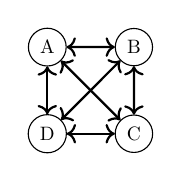
\begin{tikzpicture}[scale=0.55, every node/.style={scale=0.7}]
    \node[draw, circle, minimum size=0.6cm] (A) at (0,2) {A};
    \node[draw, circle, minimum size=0.6cm] (B) at (2,2) {B};
    \node[draw, circle, minimum size=0.6cm] (C) at (2,0) {C};
    \node[draw, circle, minimum size=0.6cm] (D) at (0,0) {D};
    \draw[<->, thick] (A) -- (B);
    \draw[<->, thick] (A) -- (C);
    \draw[<->, thick] (A) -- (D);
    \draw[<->, thick] (B) -- (C);
    \draw[<->, thick] (B) -- (D);
    \draw[<->, thick] (C) -- (D);
  \end{tikzpicture}
  }
  \hfill
  \subfloat[Hub-and-Spoke $O(N)$]{
  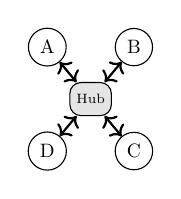
\begin{tikzpicture}[scale=0.55, every node/.style={scale=0.7}]
    \node[draw, rectangle, rounded corners, minimum size=0.6cm, fill=gray!20] (Hub) at (1,1) {\scriptsize Hub};
    \node[draw, circle, minimum size=0.6cm] (A) at (0,2.2) {A};
    \node[draw, circle, minimum size=0.6cm] (B) at (2,2.2) {B};
    \node[draw, circle, minimum size=0.6cm] (C) at (2,-0.2) {C};
    \node[draw, circle, minimum size=0.6cm] (D) at (0,-0.2) {D};
    \draw[<->, thick] (A) -- (Hub);
    \draw[<->, thick] (B) -- (Hub);
    \draw[<->, thick] (C) -- (Hub);
    \draw[<->, thick] (D) -- (Hub);
  \end{tikzpicture}
  }
  \hfill
  \subfloat[Canonical Data Model]{
  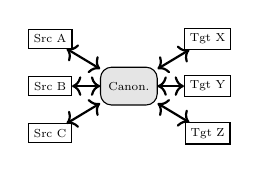
\begin{tikzpicture}[scale=0.5, every node/.style={scale=0.6}]
    \node[draw, rectangle, minimum width=0.7cm, minimum height=0.4cm] (S1) at (-1.2,1.2) {\scriptsize Src A};
    \node[draw, rectangle, minimum width=0.7cm, minimum height=0.4cm] (S2) at (-1.2,0) {\scriptsize Src B};
    \node[draw, rectangle, minimum width=0.7cm, minimum height=0.4cm] (S3) at (-1.2,-1.2) {\scriptsize Src C};
    \node[draw, rectangle, rounded corners, minimum width=1.2cm, minimum height=0.8cm, fill=gray!20] (CDM) at (0.8,0) {\scriptsize Canon.};
    \node[draw, rectangle, minimum width=0.7cm, minimum height=0.4cm] (T1) at (2.8,1.2) {\scriptsize Tgt X};
    \node[draw, rectangle, minimum width=0.7cm, minimum height=0.4cm] (T2) at (2.8,0) {\scriptsize Tgt Y};
    \node[draw, rectangle, minimum width=0.7cm, minimum height=0.4cm] (T3) at (2.8,-1.2) {\scriptsize Tgt Z};
    \draw[<->, thick] (S1) -- (CDM);
    \draw[<->, thick] (S2) -- (CDM);
    \draw[<->, thick] (S3) -- (CDM);
    \draw[<->, thick] (CDM) -- (T1);
    \draw[<->, thick] (CDM) -- (T2);
    \draw[<->, thick] (CDM) -- (T3);
  \end{tikzpicture}
  }
  \caption{Point-to-point integration, Hub-and-Spoke integration, and the role of a canonical data model}
  \label{fig:integration-patterns}
\end{figure}




\section{M-Model\textsuperscript{+}}
\label{sec:unified-meta-schema}

SMILE requires a canonical schema representation that can serve both as the semantic basis of the language and as the intermediate representation of the migration pipeline. Although the M-Model~\cite{conrad2022metamodels} already provides a suitable foundation for cross-paradigm migration, it does not yet capture all constructs required by the operation taxonomy introduced in Section~\ref{sec:operation-taxonomy}. In particular, SMILE must represent graph-specific labels, paradigm-dependent key semantics, attribute-level schema properties, and structurally different relationship forms within one common representation. M-Model\textsuperscript{+} therefore extends the original M-Model in three directions.
At the attribute level, it adds \texttt{is\_key}, \texttt{is\_optional}, and extended key types such as \texttt{NODE\_KEY} and \texttt{DOCUMENT\_ID} so that labels, key participation, and nullability become explicit schema properties.
At the type level, it introduces \texttt{TupleDataType} for Cassandra's \texttt{tuple<>} and adds \texttt{labels} on \texttt{EntityType} for graph and document identifiers.
At the relationship level, it distinguishes three subtypes of \texttt{Relationship}, namely \texttt{Reference}, \texttt{Embedded}, and \texttt{Edge}, so that relational foreign keys, embedded document structures, and graph edges fit within one shared model.
Figure~\ref{fig:meta-schema} shows these additions, where black elements originate from the M-Model and blue elements denote SMILE-specific extensions.

\begin{figure}[t]
  \centering
  \resizebox{\columnwidth}{!}{%
  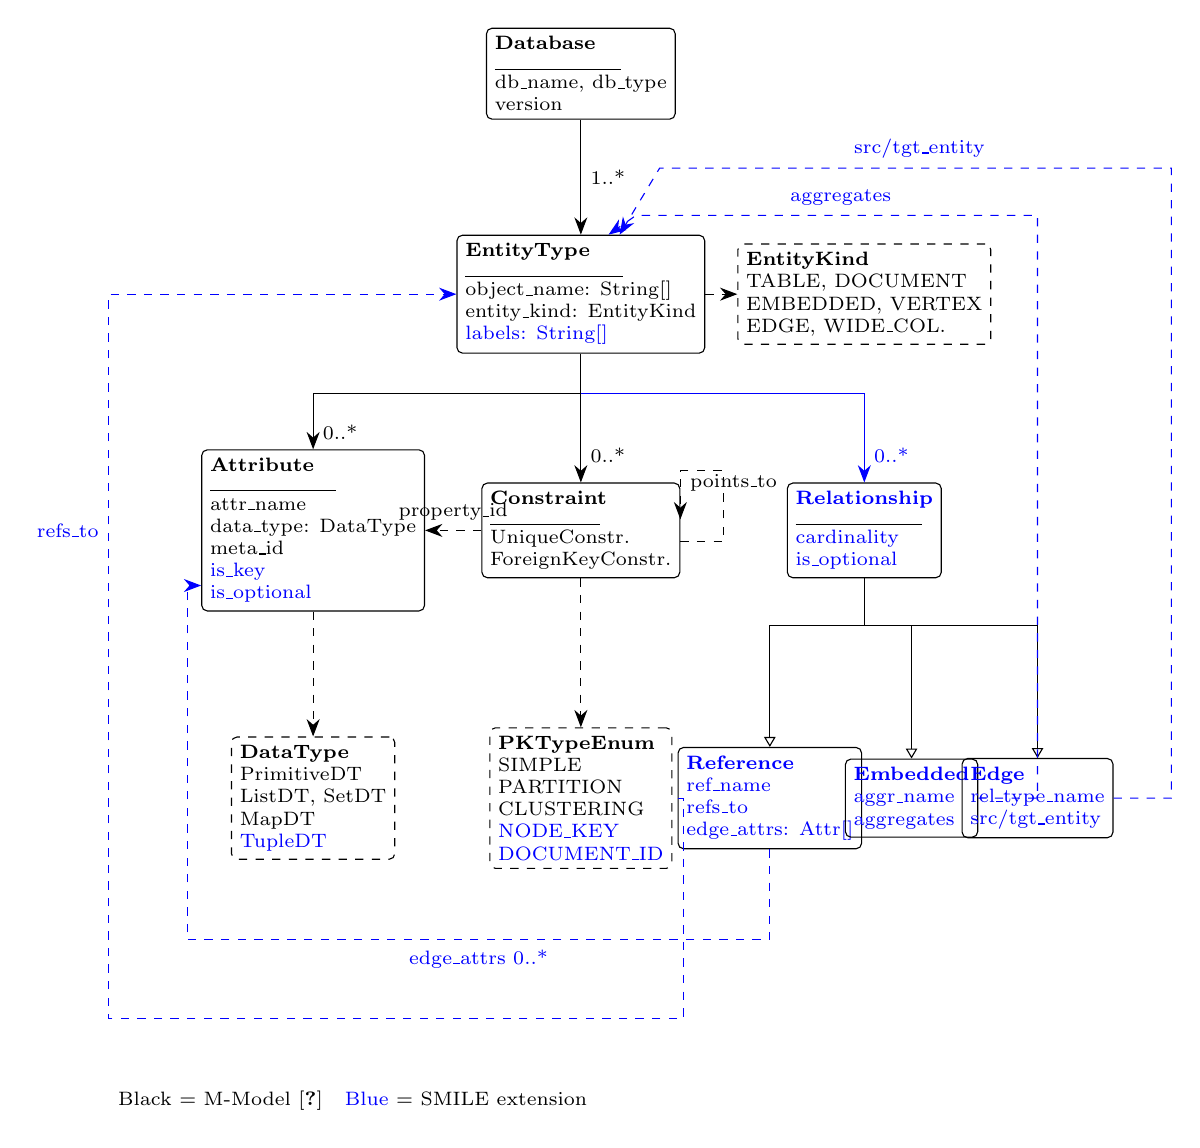
\begin{tikzpicture}[
    >={Stealth[length=2.2mm]},
    cls/.style={draw, rounded corners=2pt, align=left,
                inner sep=3pt, font=\scriptsize},
    enu/.style={draw, dashed, rounded corners=2pt,
                align=left, inner sep=3pt, font=\scriptsize},
    sub/.style={draw, rounded corners=2pt, align=left,
                inner sep=3pt, font=\scriptsize},
    lbl/.style={font=\scriptsize},
  ]

  % ============ Row 0: Database ============
  \node[cls] (db) at (0,0) {
    \textbf{Database}\\[-1pt]
    {\rule{1.6cm}{0.2pt}}\\[-1pt]
    db\_name, db\_type\\
    version
  };

  % ============ Row 1: EntityType ============
  \node[cls] (et) at (0,-2.8) {
    \textbf{EntityType}\\[-1pt]
    {\rule{2.0cm}{0.2pt}}\\[-1pt]
    object\_name: String[]\\
    entity\_kind: EntityKind\\
    \textcolor{blue}{labels: String[]}
  };

  % ============ EntityKind ============
  \node[enu] (ek) at (3.6,-2.8) {
    \textbf{EntityKind}\\
    TABLE, DOCUMENT\\
    EMBEDDED, VERTEX\\
    EDGE, WIDE\_COL.
  };

  % ============ Row 2 ============
  \node[cls] (attr) at (-3.4,-5.8) {
    \textbf{Attribute}\\[-1pt]
    {\rule{1.6cm}{0.2pt}}\\[-1pt]
    attr\_name\\
    data\_type: DataType\\
    meta\_id\\
    \textcolor{blue}{is\_key}\\
    \textcolor{blue}{is\_optional}
  };

  \node[cls] (con) at (0,-5.8) {
    \textbf{Constraint}\\[-1pt]
    {\rule{1.4cm}{0.2pt}}\\[-1pt]
    UniqueConstr.\\
    ForeignKeyConstr.
  };

  \node[cls] (rel) at (3.6,-5.8) {
    \textcolor{blue}{\textbf{Relationship}}\\[-1pt]
    {\rule{1.6cm}{0.2pt}}\\[-1pt]
    \textcolor{blue}{cardinality}\\
    \textcolor{blue}{is\_optional}
  };

  % ============ Row 3 ============
  \node[enu] (dt) at (-3.4,-9.2) {
    \textbf{DataType}\\
    PrimitiveDT\\
    ListDT, SetDT\\
    MapDT\\
    \textcolor{blue}{TupleDT}
  };

  \node[enu] (pk) at (0,-9.2) {
    \textbf{PKTypeEnum}\\
    SIMPLE\\
    PARTITION\\
    CLUSTERING\\
    \textcolor{blue}{NODE\_KEY}\\
    \textcolor{blue}{DOCUMENT\_ID}
  };

  \node[sub] (ref) at (2.4,-9.2) {
    \textcolor{blue}{\textbf{Reference}}\\
    \textcolor{blue}{ref\_name}\\
    \textcolor{blue}{refs\_to}\\
    \textcolor{blue}{edge\_attrs: Attr[]}
  };
  \node[sub] (emb) at (4.2,-9.2) {
    \textcolor{blue}{\textbf{Embedded}}\\
    \textcolor{blue}{aggr\_name}\\
    \textcolor{blue}{aggregates}
  };
  \node[sub] (edge) at (5.8,-9.2) {
    \textcolor{blue}{\textbf{Edge}}\\
    \textcolor{blue}{rel\_type\_name}\\
    \textcolor{blue}{src/tgt\_entity}
  };

  % ======== SOLID CONNECTIONS ========

  \draw[->] (db.south) -- node[right, lbl] {1..*} (et.north);

  \draw[dashed, ->] (et.east) -- (ek.west);

  \draw (et.south) -- ++(0,-0.5) coordinate (etfork);
  \draw[->] (etfork) -| node[pos=0.85, right, lbl] {0..*} (attr.north);
  \draw[->] (etfork) -| node[pos=0.85, right, lbl] {0..*} (con.north);
  \draw[->, blue] (etfork) -| node[pos=0.85, right, lbl] {\textcolor{blue}{0..*}} (rel.north);

  \draw[dashed, ->] (attr.south) -- (dt.north);
  \draw[dashed, ->] (con.south) -- (pk.north);

  \draw[dashed, ->] (con.west) -- node[above, lbl] {property\_id} (attr.east);

  \draw[dashed, ->] ([yshift=-4pt]con.east)
    -- ++(0.55,0) -- ++(0,0.9) -- ++(-0.55,0) -- ([yshift=4pt]con.east)
    node[right, lbl, pos=0.25] {points\_to};

  \draw (rel.south) -- ++(0,-0.6) coordinate (relfork);
  \draw[-{Triangle[open]}] (relfork) -| (ref.north);
  \draw[-{Triangle[open]}] (relfork) -| (emb.north);
  \draw[-{Triangle[open]}] (relfork) -| (edge.north);

  % ======== BLUE DASHED ========

  % 1) edge_attrs: ref.south -> down -> left PAST DataType -> up -> attr.west
  %    Routes around DataType on the LEFT side
  \draw[dashed, ->, blue]
    (ref.south)
    -- (ref.south |- 0,-11.0)
    -- (-5.0,-11.0)
    -- (-5.0,-6.5)
    -- (attr.west |- 0,-6.5);
  \node[below, lbl, blue] at (-1.3,-11.0) {edge\_attrs 0..*};

  % 2) refs_to: ref.west -> down below edge_attrs -> far left -> up -> et.west
  \draw[dashed, ->, blue]
    (ref.west)
    -- (1.3,-9.2 |- ref.west)
    -- (1.3,-12.0)
    -- (-6.0,-12.0)
    -- (-6.0,-2.8)
    -- (et.west);
  \node[left, lbl, blue] at (-6.0,-5.8) {refs\_to};

  % 3) aggregates: right channel x=5.8, top at y=-1.8
  \draw[dashed, ->, blue]
    (emb.east)
    -- (5.8,-9.2 |- emb.east)
    -- (5.8,-1.8)
    -- (0.7,-1.8)
    -- ([xshift=10pt]et.north);
  \node[above, lbl, blue] at (3.3,-1.8) {aggregates};

  % 4) src/tgt_entity: far right channel x=7.5, top at y=-1.2
  \draw[dashed, ->, blue]
    (edge.east)
    -- (7.5,-9.2 |- edge.east)
    -- (7.5,-1.2)
    -- (1.0,-1.2)
    -- ([xshift=14pt]et.north);
  \node[above, lbl, blue] at (4.3,-1.2) {src/tgt\_entity};

  % ============ Legend ============
  \node[lbl, anchor=north west] at (-6.0,-12.8) {
    Black = M-Model~\cite{conrad2022metamodels}\quad
    \textcolor{blue}{Blue} = SMILE extension
  };

  \end{tikzpicture}
  }% end resizebox
  \caption{M-Model\textsuperscript{+}: M-Model (black) with SMILE extensions ({\textcolor{blue}{blue}})}
  \label{fig:meta-schema}
\end{figure}


\paragraph{Rationale and Relation to Prior Work.}
The M-Model is used as the basis of M-Model\textsuperscript{+} because it aligns more directly with the transformation requirements of SMILE than alternative metamodels such as U-Schema (Table~\ref{tab:metamodel-comparison-rw}). In particular, its unified relationship hierarchy allows references, embedded structures, and graph edges to be treated within one common framework, while its explicit key typing already captures distinctions required by wide-column systems. These properties make it a suitable starting point for a canonical hub representation in a Hub-and-Spoke architecture.

The M-Model already covers the four target paradigms and provides a unified relationship hierarchy, which gives M-Model\textsuperscript{+} a solid foundation. The extensions introduced above add the constructs that SMILE manipulates directly, such as graph-specific labels, typed key semantics, and attribute-level schema properties, so that these features are preserved throughout reverse engineering, transformation, and forward engineering. M-Model\textsuperscript{+} therefore builds on the M-Model as a targeted refinement for cross-paradigm schema change.

% ============================================================
\section{Implementation}
\label{sec:implementation}
% ============================================================

The SMILE Engine separates paradigm-specific schema handling from paradigm-independent transformation semantics.
Schema changes are defined once over M-Model\textsuperscript{+} and reused across source--target pairs, new database systems can be added through a single adapter, and validation runs independently of execution so that script errors and adapter errors can be traced separately.
The implementation combines a layered architecture with a pipeline that routes all transformations through the canonical metamodel.

\subsection{System Architecture}

\begin{figure}[t]
  \centering
  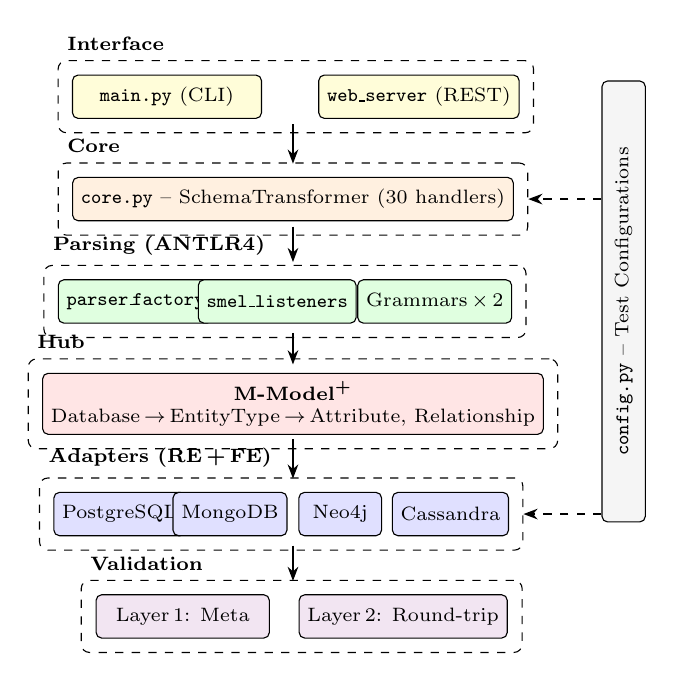
\begin{tikzpicture}[
    font=\scriptsize,
    mod/.style={draw, rounded corners=2pt, minimum height=0.55cm,
                align=center, inner sep=3pt},
    lyr/.style={draw, dashed, rounded corners=3pt,
                minimum width=5.6cm, inner sep=5pt},
    arr/.style={-{Stealth[length=1.8mm]}, semithick},
    lbl/.style={font=\scriptsize\bfseries, anchor=south west},
  ]

  \def\cx{2.4}

  % -- Layer 1: Interface
  \node[mod, fill=yellow!15, minimum width=2.4cm] (cli) at (0.8, 0)
    {\texttt{main.py} (CLI)};
  \node[mod, fill=yellow!15, minimum width=2.4cm] (web) at (4.0, 0)
    {\texttt{web\_server} (REST)};
  \node[lyr, fit=(cli)(web), label={[lbl]north west:Interface}] (L1) {};

  % -- Layer 2: Core
  \node[mod, fill=orange!12, minimum width=5.0cm] (core) at (\cx, -1.3)
    {\texttt{core.py} -- SchemaTransformer (30 handlers)};
  \node[lyr, fit=(core), label={[lbl]north west:Core}] (L2) {};

  % -- Layer 3: Parsing
  \node[mod, fill=green!12, minimum width=1.4cm] (pf) at (0.4, -2.6)
    {\texttt{parser\_\!factory}};
  \node[mod, fill=green!12, minimum width=1.6cm] (sl) at (2.2, -2.6)
    {\texttt{smel\_listeners}};
  \node[mod, fill=green!12, minimum width=1.4cm] (gr) at (4.2, -2.6)
    {Grammars\,$\times$\,2};
  \node[lyr, fit=(pf)(sl)(gr),
        label={[lbl]north west:Parsing (ANTLR4)}] (L3) {};

  % -- Layer 4: Unified Meta Schema
  \node[mod, fill=red!10, minimum width=5.0cm, minimum height=0.7cm]
    (meta) at (\cx, -3.9)
    {\textbf{M-Model\textsuperscript{+}}\\
     Database\,$\rightarrow$\,EntityType\,$\rightarrow$\,%
     Attribute, Relationship};
  \node[lyr, fit=(meta), label={[lbl]north west:Hub}] (L4) {};

  % -- Layer 5: Adapters
  \node[mod, fill=blue!12, minimum width=1.05cm] (pg) at (0.2, -5.3)
    {PostgreSQL};
  \node[mod, fill=blue!12, minimum width=1.05cm] (mg) at (1.6, -5.3)
    {MongoDB};
  \node[mod, fill=blue!12, minimum width=1.05cm] (nj) at (3.0, -5.3)
    {Neo4j};
  \node[mod, fill=blue!12, minimum width=1.05cm] (ca) at (4.4, -5.3)
    {Cassandra};
  \node[lyr, fit=(pg)(mg)(nj)(ca),
        label={[lbl]north west:Adapters (RE\,+\,FE)}] (L5) {};

  % -- Layer 6: Validation
  \node[mod, fill=violet!10, minimum width=2.2cm] (vl1) at (1.0, -6.6)
    {Layer\,1: Meta};
  \node[mod, fill=violet!10, minimum width=2.2cm] (vl2) at (3.8, -6.6)
    {Layer\,2: Round-trip};
  \node[lyr, fit=(vl1)(vl2),
        label={[lbl]north west:Validation}] (L6) {};

  % -- Side: Config (cross-cutting)
  \node[draw, rounded corners=2pt, fill=gray!8,
        minimum height=5.6cm, minimum width=0.55cm,
        align=center, inner sep=2pt] (cfg) at (6.6, -2.6)
    {\rotatebox{90}{\texttt{config.py} -- Test Configurations}};

  % -- Vertical arrows (layer to layer)
  \draw[arr] (\cx, -0.35) -- (\cx, -0.85);
  \draw[arr] (\cx, -1.65) -- (\cx, -2.10);
  \draw[arr] (\cx, -3.00) -- (\cx, -3.40);
  \draw[arr] (\cx, -4.35) -- (\cx, -4.85);
  \draw[arr] (\cx, -5.70) -- (\cx, -6.15);

  % -- Config side arrows (dashed, horizontal)
  \draw[arr, dashed] (cfg.west |- L2.east) -- (L2.east);
  \draw[arr, dashed] (cfg.west |- L5.east) -- (L5.east);

  \end{tikzpicture}
  \caption{SMILE Engine architecture: six layers with M-Model\textsuperscript{+} as central hub}
  \label{fig:system-architecture}
\end{figure}




The prototype is implemented in Python~3.13 with ANTLR4 for parser generation.\footnote{The prototype implementation is available at \url{https://github.com/baobaodaren0918/SMILE-3.0}.}
The system follows a layered architecture~\cite{richards2020fundamentals}, not because layering is unusual, but because the involved concerns differ fundamentally in their degree of reuse.
Database-native parsing and export logic are specific to individual systems and therefore belong at the boundaries.
Transformation semantics, by contrast, must remain stable across migration and evolution scenarios and are therefore concentrated in a shared core.

The \emph{interface layer} provides both a command-line interface and a REST-based web interface.
The command-line interface supports repeatable batch execution, which simplifies evaluation and regression testing.
The web interface serves a different purpose and allows users to inspect migration results interactively, including generated schemas, execution logs, and validation outcomes.
This separation reflects the dual role of the engine as both an experimental prototype and an interactive demonstration environment.

The \emph{core layer} contains the \texttt{SchemaTransformer}, which implements the semantics of SMILE operations through dedicated handlers.
All handlers operate on M-Model\textsuperscript{+}, not on database-native schemas.
As a result, the same transformation logic can be reused regardless of whether the source schema originates from PostgreSQL, MongoDB, Neo4j, or Cassandra.
This paradigm-independent execution model is essential because SMILE is intended to cover both intra-system evolution and inter-system migration within one operation framework.

The \emph{parsing layer} isolates concrete syntax from execution semantics.
A \texttt{parser\_factory} selects the appropriate grammar variant based on the file extension, and \texttt{smel\_listeners}\footnote{The implementation retains the earlier working title \emph{SMEL} in file and module names (e.g., \texttt{.smel} extension, \texttt{smel\_listeners.py}); the language was subsequently renamed to SMILE.} translate the parse tree into an ordered list of operations.
This design allows the Specific and Generalized grammars to remain distinct at the syntax level while converging to the same internal representation.
The engine therefore supports multiple surface notations without duplicating semantic logic.

The \emph{hub layer} consists of M-Model\textsuperscript{+}, which serves as the canonical intermediate representation for the entire system.
All other layers interact through this representation.
Once a source schema has been mapped into the canonical model, transformation, validation, and export no longer depend on the original database format.
The metamodel therefore serves as the semantic center of the implementation.

The \emph{adapter layer} contains one adapter per supported database system.
Each adapter combines reverse engineering and forward engineering in the same module.
Keeping both directions together reduces redundancy and helps maintain consistency between how a system is parsed and how it is generated again.
Round-trip validation relies on this consistency, since export correctness depends directly on the assumptions made during parsing.

The \emph{validation layer} runs independently of transformation execution.
A failed result may stem from an incorrect SMILE script or from a bug in the target adapter; keeping validation separate lets the engine pinpoint which part is at fault.

\texttt{config.py} complements the layered architecture as a cross-cutting configuration component.
It stores the migration and evolution definitions used to instantiate concrete runs, including source files, SMILE scripts, and source/target types.

\subsection{Pipeline Stages}
\label{sec:pipeline-stages}

The SMILE Engine executes schema change as a five-phase pipeline that connects native source schemas, SMILE scripts, the canonical metamodel, and native target schemas.
Figure~\ref{fig:architecture} summarizes this process.
Conceptually, the pipeline combines two input streams.
One stream converts the source schema into M-Model\textsuperscript{+}, while the other translates the SMILE script into an ordered transformation program.
Both streams meet in the transformation core and are reconciled again during export and validation.

\begin{figure*}[t]
  \centering
  \includegraphics[width=\textwidth]{gfx/pipeline1.drawio.pdf}
  \caption{SMILE five-phase migration pipeline from source schema to target delivery}
  \label{fig:architecture}
\end{figure*}

\textbf{Phase~1 (Input).}
Execution starts from two inputs: a native source schema and a SMILE script written in either the Specific or the Generalized grammar.

\textbf{Phase~2 (Parsing and Reverse Engineering).}
The two inputs are processed in parallel.
On the schema side, the source adapter reverse-engineers the native schema into M-Model\textsuperscript{+}.
Top-level structures such as tables, collections, vertices, or column families are mapped to \texttt{EntityType} objects, while relationships are represented as \texttt{Reference}, \texttt{Embedded}, or \texttt{Edge} according to their source semantics.
Native data types are translated into the shared data-type system of the metamodel.
This step removes database-specific representational differences before any transformation logic is applied.

On the script side, the parsing layer turns the SMILE program into an ordered list of \texttt{Operation} objects.
Although the Specific and Generalized grammars differ at the concrete-syntax level, they converge here to the same internal representation, so that syntax variation does not affect execution semantics.

\textbf{Phase~3 (Execution).}
The \texttt{SchemaTransformer} applies the generated operation list to the reverse-engineered source schema represented in M-Model\textsuperscript{+}.
Each operation is dispatched to a dedicated handler implementing the taxonomy defined in Section~\ref{sec:operation-taxonomy}.
Because handlers operate over the canonical metamodel, the execution model remains independent of the concrete source and target systems.

After the scripted operations have been applied, an additional normalization step aligns entity kinds with the target paradigm while preserving graph-specific semantics where required, for example for \texttt{EDGE} entities.
The result of this phase is Meta~V2, i.e., the transformed target schema in canonical form.

\textbf{Phase~4 (Forward Engineering and Validation).}
The target adapter exports Meta~V2 into the native schema definition language of the target system.
For relational targets this results in PostgreSQL DDL, for document targets in MongoDB JSON Schema, for graph targets in Cypher constraints, and for wide-column targets in Cassandra CQL.
Reverse engineering and forward engineering are co-located in the same adapter module, which keeps export logic aligned with the structural assumptions used during parsing.

Validation is integrated at this stage but remains conceptually separate from execution.
Layer~1 validates script correctness by comparing Meta~V2 against the expected target schema obtained by parsing an independently authored ground-truth target file.
Layer~2 validates adapter correctness by reverse-engineering the exported target schema and comparing the resulting round-trip meta representation against the same expected target schema.
This two-layer structure makes it possible to distinguish errors in the transformation script from errors in target-schema generation.

\textbf{Phase~5 (Delivery).}
The generated target schema, execution log, and validation results are exposed through the user interface, where source and target schemas can be inspected side by side together with the executed operations and validation feedback.

\section{Evaluation}
\label{sec:evaluation}

\begin{figure*}[t]
\centering
\resizebox{\textwidth}{!}{%
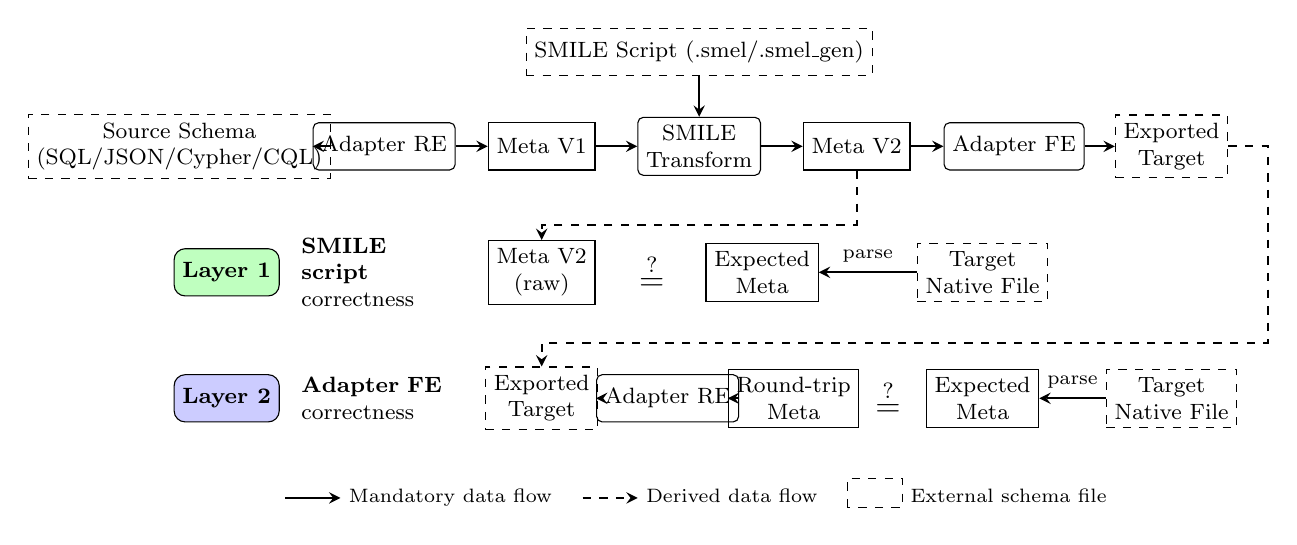
\begin{tikzpicture}[
  font=\footnotesize,
  box/.style={draw, rectangle, rounded corners=2pt, minimum height=0.6cm,
              align=center, inner sep=3pt},
  data/.style={draw, rectangle, minimum height=0.6cm,
               align=center, inner sep=3pt},
  file/.style={draw, rectangle, dashed, minimum height=0.6cm,
               align=center, inner sep=3pt},
  layer/.style={draw, rectangle, rounded corners=4pt, fill=#1,
                minimum height=0.6cm, minimum width=1.1cm,
                align=center, inner sep=3pt, font=\footnotesize\bfseries},
  arr/.style={->, >=stealth, thick},
  darr/.style={->, >=stealth, thick, dashed},
]
%% Top row
\node[file]  at (0,   0) (src)  {Source Schema\\(SQL/JSON/Cypher/CQL)};
\node[box]   at (2.6, 0) (re)   {Adapter RE};
\node[data]  at (4.6, 0) (v1)   {Meta V1};
\node[box]   at (6.6, 0) (sml)  {SMILE\\Transform};
\node[data]  at (8.6, 0) (v2)   {Meta V2};
\node[box]   at (10.6,0) (fe)   {Adapter FE};
\node[file]  at (12.6,0) (exp)  {Exported\\Target};
\draw[arr] (src) -- (re);
\draw[arr] (re)  -- (v1);
\draw[arr] (v1)  -- (sml);
\draw[arr] (sml) -- (v2);
\draw[arr] (v2)  -- (fe);
\draw[arr] (fe)  -- (exp);
\node[file] at (6.6, 1.2) (script) {SMILE Script (.smel/.smel\_gen)};
\draw[arr] (script) -- (sml);
%% Layer 1
\node[layer=green!25] at (0.6,-1.6) (l1) {Layer 1};
\node[right=0.15cm of l1, font=\footnotesize, text width=1.9cm, align=left]
  {\textbf{SMILE script}\\correctness};
\node[data] at (4.6,-1.6)  (l1v2)   {Meta V2\\(raw)};
\node       at (6.0,-1.6)           {\large$\stackrel{?}{=}$};
\node[data] at (7.4,-1.6)  (l1exp)  {Expected\\Meta};
\node[file] at (10.2,-1.6) (l1file) {Target\\Native File};
\draw[darr] (v2.south) -- (8.6,-1.0) -- (4.6,-1.0) -- (l1v2.north);
\draw[arr]  (l1file) -- node[above,font=\scriptsize]{parse} (l1exp);
%% Layer 2
\node[layer=blue!20] at (0.6,-3.2) (l2) {Layer 2};
\node[right=0.15cm of l2, font=\footnotesize, text width=1.9cm, align=left]
  {\textbf{Adapter FE}\\correctness};
\node[file] at (4.6,-3.2)  (l2src)  {Exported\\Target};
\node[box]  at (6.2,-3.2)  (l2re)   {Adapter RE};
\node[data] at (7.8,-3.2)  (l2rt)   {Round-trip\\Meta};
\node       at (9.0,-3.2)           {\large$\stackrel{?}{=}$};
\node[data] at (10.2,-3.2) (l2exp)  {Expected\\Meta};
\node[file] at (12.6,-3.2) (l2file) {Target\\Native File};
\draw[darr] (exp.east) -- ++(0.5,0) -- ++(0,-2.5) -- (4.6,-2.5) -- (l2src.north);
\draw[arr]  (l2src) -- (l2re);
\draw[arr]  (l2re)  -- (l2rt);
\draw[arr]  (l2file)-- node[above,font=\scriptsize]{parse} (l2exp);
%% Legend
\node[align=left, font=\scriptsize] at (6.6,-4.4) {%
  \tikz[baseline=-0.5ex]{\draw[->,>=stealth,thick](0,0)--(0.7,0);}~Mandatory data flow \quad
  \tikz[baseline=-0.5ex]{\draw[->,>=stealth,thick,dashed](0,0)--(0.7,0);}~Derived data flow \quad
  \tikz[baseline=-0.5ex]{\draw[dashed](0,-0.12) rectangle (0.7,0.25);}~External schema file
};
\end{tikzpicture}%
}%
\caption{Two-layer validation pipeline}
\label{fig:validation-pipeline}
\end{figure*}

We evaluate whether SMILE can express and execute schema
changes consistently across the full $4 \times 4$ scenario matrix and
whether target export preserves that consistency.
To this end, we consider all 16 directions, comprising
4 intra-system evolution cases and 12 inter-system migration
cases, and instantiate each of them in both grammar variants.

As a common schema basis we use a subset of the Northwind
dataset comprising 8~entities (e.g., \texttt{orders},
\texttt{products}, \texttt{employees}), 69~attributes, and
8~foreign-key relationships including one self-reference and
one composite primary key. These entities were selected to
cover the structural patterns most relevant to cross-paradigm
migration, such as multi-table foreign-key chains, nested
address fields, self-referential hierarchies, and composite
keys. Each paradigm has its own native representation of this
subset, and applying both grammar variants across all
directions yields 32 test configurations in total.
Every configuration is assessed through execution and a
two-layer validation procedure (Figure~\ref{fig:validation-pipeline}).

For cross-model migrations, the four original Northwind schema files form a closed validation loop.
Each native schema acts both as the source of outgoing migrations and as the expected target of incoming migrations from the other paradigms.
Because these target schemas are independently authored, the evaluation does not rely on manually constructed expected outputs.

Layer~1 validates the correctness of the schema change expressed in SMILE.
It compares the transformed canonical schema (Meta~V2) with the expected target schema obtained by reverse-engineering the corresponding ground-truth target file.
This layer therefore tests whether the script semantics produce the intended structural result independently of any target export.

Layer~2 validates the faithfulness of target export.
It reverse-engineers the schema generated by the target adapter and compares the resulting round-trip meta representation with the same expected target schema.


%/The results are listed in Table~\ref{tab:eval-results}.
\begin{table}[t]
\centering
\caption{Validation results across 32 Northwind test scripts.}
\label{tab:eval-results}
\renewcommand{\arraystretch}{1.15}
\begin{tabular}{l c c c c}
\toprule
\textbf{Category} & \textbf{Configs} & \textbf{Layer 1} & \textbf{Layer 2} & \textbf{Notices} \\
\midrule
Same-model          & 8  & 8/8   & 8/8   & 4  \\
Cross-model         & 24 & 24/24 & 24/24 & 14 \\
\midrule
\textbf{Total}      & \textbf{32} & \textbf{32/32} & \textbf{32/32} & \textbf{18} \\
\bottomrule
\end{tabular}
\end{table}

All 32 configurations (8 same-model, 24 cross-model) pass both validation layers.
Across both validation layers, the only differences recorded are 18 \texttt{is\_optional} notices (4 in same-model cases and 14 in cross-model cases), caused by paradigm-specific nullability defaults rather than incorrect transformations.
For example, Cassandra clustering keys are inherently \texttt{NOT NULL}, whereas the corresponding attribute may be nullable in a relational or document source.
These notices do not invalidate the structural result but expose residual semantic gaps in cross-paradigm migration.
% ============================================================
\section{Conclusion}
\label{sec:conclusion}
% ============================================================

This paper introduced SMILE, a domain-specific language for schema evolution and schema migration across relational, document, graph, and wide-column databases.

At its core, SMILE provides a common operation model for schema change across paradigms.
This model is realized through a taxonomy of atomic schema change primitives and two grammar variants that share the same semantics while supporting different concrete syntactic styles.
In this way, the approach connects intra-system evolution and inter-system migration within one language framework and covers all 16 directions of the $4 \times 4$ scenario matrix.

The approach further relies on M-Model\textsuperscript{+} as a canonical hub representation for cross-paradigm schema migration.
Schema changes are expressed and executed over this shared abstraction, replacing pairwise mappings between individual systems.
The SMILE Engine implements this workflow through adapters for
PostgreSQL, MongoDB, Neo4j, and Cassandra, with integrated validation
and a web-based interface for inspecting migration results.

The evaluation across 32 Northwind configurations indicates that the approach can be applied consistently across all four paradigms and all migration and evolution directions considered in this work.
The two-layer validation design further demonstrates that transformation correctness and adapter correctness can be assessed separately, which is an important property for a language-centered migration framework.

The 32/32 pass rate across both grammar variants and all 16 directions suggests that SMILE provides a workable basis for cross-paradigm schema change.

\textbf{Limitations.}
SMILE is limited to schema-level change and therefore does not address the data-migration logic that often accompanies practical migration scenarios.
Its current modeling scope is also narrower for document stores, since the MongoDB adapter assumes one root structure per collection and does not represent structural variation within the same collection.
In addition, the framework currently supports one-shot schema change rather than version-aware evolution, and the nullability notices observed in the evaluation show that some cross-paradigm semantic mismatches still require manual review.

\textbf{Future work.}
Future work includes extending SMILE beyond schema-level migration toward combined schema and data migration, for example by generating executable ETL specifications alongside schema scripts.
Another direction is to support version-aware evolution, including schema histories and incremental transformations.
We also plan to improve authoring and automation support, ranging from IDE integration through Language Server Protocol features to the use of large language models for generating SMILE scripts from natural-language migration requirements.



\begin{acks}
The work of Dominique Hausler has been funded by Deutsche Forschungsgemeinschaft (German Research Foundation) -- 552691270.
\end{acks}

\section*{Declaration on Generative AI}
The logo was generated with DALL-E 3. ChatGPT and AI Studio were used for rephrasing and to find synonyms.

\bibliographystyle{ACM-Reference-Format}
\bibliography{bibliography}

\end{document}
